\section{Crowd-Shared Wireless Mesh Networks}
\label{sec:architecture}

The underlying problem with PAWS or any crowd-shared network is that they serve as single point of Internet access to guest users within the coverage of the wireless router and hence, they have no provision to extend the coverage when no bandwidth is being shared. Based on our experience from the trial PAWS deployment, PAWS routers were always not available for certain periods, because sharers needed all the bandwidth of their broadband connection or due to other reasons, such as economic constraints placed on home users in underprivileged areas where they are forced to conserve energy by turning off the routers at nights. In this respect, Fig. \ref{fig:paws-avail} presents a six-month view of the PAWS routers status (available/unavailable) logs demonstrating that not a single router was available continuously over the entire duration. These observed user behaviors entail significant challenges for the successful adoption of PAWS. 

\begin{figure}[t]
\begin{center}
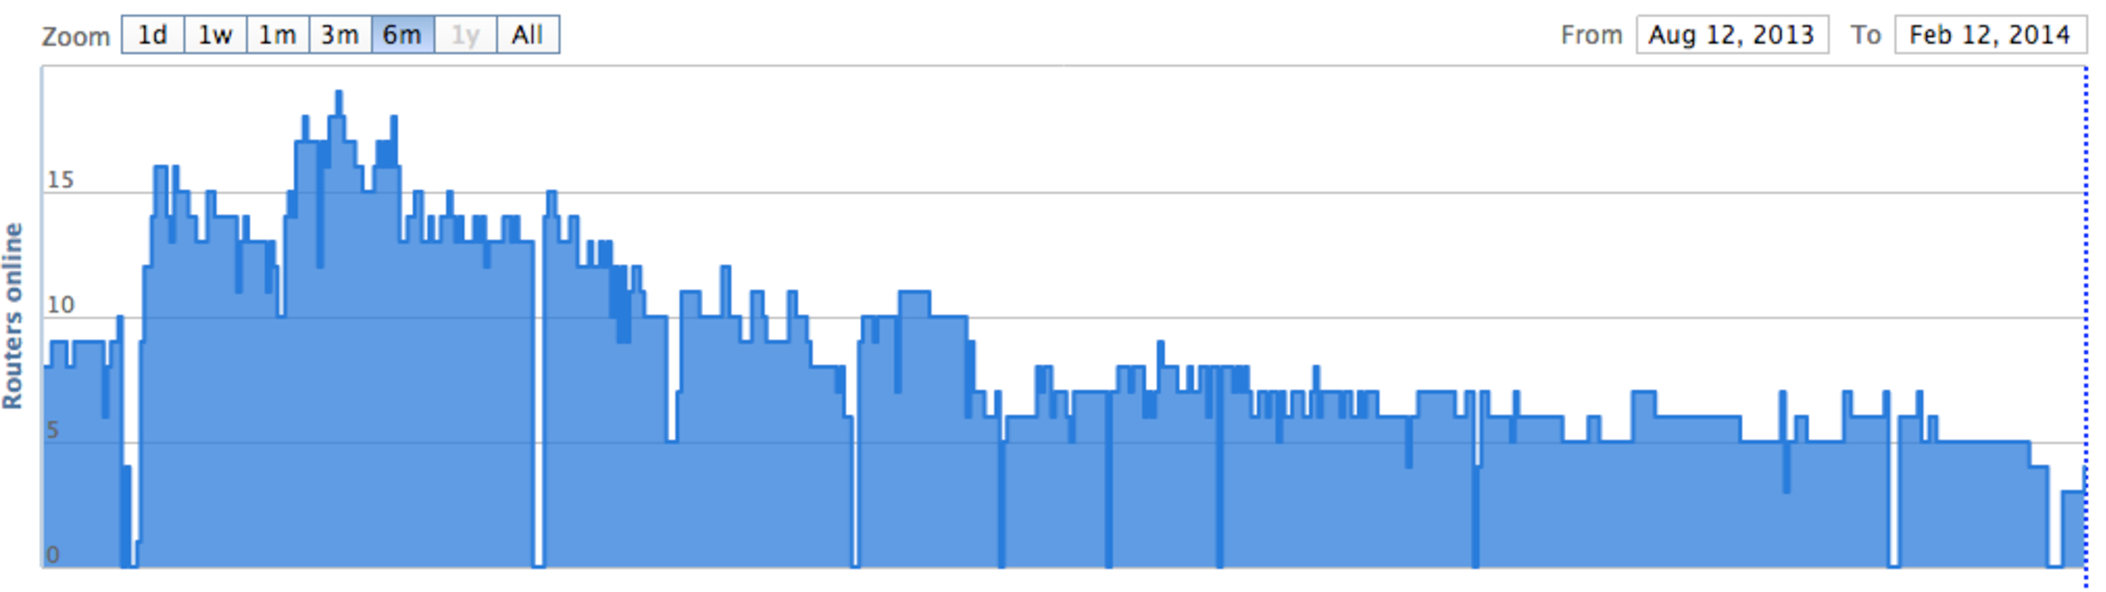
\includegraphics[width=1\linewidth]{paws-avail.pdf}  
\caption{PAWS routers availability.}
\label{fig:paws-avail}
\end{center}
\end{figure}

\subsection{Crowd-Shared WMN Management}
\label{architecture:management}

A potential solution to this problem is to extend the PAWS network as a crowd-shared WMN. Such a network would allow home network users to share part of their own broadband connection to the public for free while also connected to each other as a WMN providing extended coverage. Extending PAWS to a crowd-shared WMN departs from the norm: multiple users from different ISPs form part of the WMN to provide free Internet connectivity, while most wireless community WMNs today are operated by a single organization. This raises important questions regarding the operation, configuration, and management of crowd-shared WMNs.  

SDN can facilitate the management and operation of wireless networks at large scale. Leveraging on SDN's centralized control and network-wide visibility, the management and operation of a crowd-shared WMN can be outsourced to a third party. In \cite{EWSDN}, we describe a holistic approach of coupling both social and economic incentives in designing future networks allowing the extension of the stakeholder value chain to include more than the two traditional parties (consumer and Internet service provider). Such an approach would provide opportunities for non-governmental organizations and local governments (driven by social goals rather than economic) to become virtual network operators. Enabling a third party to federate such wireless home networks would reduce the operating expenditures for network operators as well as enable new economic models for revenue creation from currently underutilized infrastructures. In particular, we rely on SDN to create the notion of Virtual Public Networks (VPuN), i.e., crowd-shared home networks created, deployed and managed through an evolutionary SDN control abstraction \cite{EWSDN}. Although originally intended for crowd-shared wireless networks such as PAWS, VPuN can also facilitate management of crowd-shared WMNs, enabling resource pooling across multiple home broadband connections depending on prevailing network conditions and usage sharing patterns. 

\subsection{Traffic Redirection}
\label{architecture:redirection}



